\documentclass[11pt]{article}

\usepackage{graphicx}
\usepackage[top=25mm, bottom=25mm, left=25mm, right=25mm, a4paper]{geometry}
\usepackage{amsmath}
\usepackage{enumitem}
\usepackage{float}
\usepackage{fancyhdr}
\usepackage{booktabs}
\usepackage{tikz}
\usepackage{steinmetz}
\usepackage{pgfplots}

\pagestyle{fancy}
\fancyhf{}
\fancyhead[R]{Baturay Kafkas - 2240357068 - Electrical \& Electronics Engineering}

\rfoot{\thepage}
\renewcommand{\headrulewidth}{0pt} 
\renewcommand{\footrulewidth}{0pt}
\sloppy

\begin{document}

\begin{center}
\large
\textbf{ELE214 - Electronics Laboratory I Preliminary Work 5}
\end{center}

\section{Questions}

\begin{enumerate}[leftmargin=*,label=\textbf{\arabic*.}]

\item Explain how you can determine the type of a MOSFET (n-- or p--channel) and test whether it is defective or not.

\item Sketch $I_D-V_{DS}$ graph for $V_{GS}= 1.2, 1.4, 1.6,\ldots, 2.2$ V.

\item Sketch $I_D-V_{GS}$ graph, indicate $V_{TH}$ using output characteristics.

\end{enumerate}

\textbf{Experimental Work (Simulation of 1-3)}

\vspace{1em}

\begin{minipage}{0.4\textwidth}
    \begin{figure}[H]
        \centering
        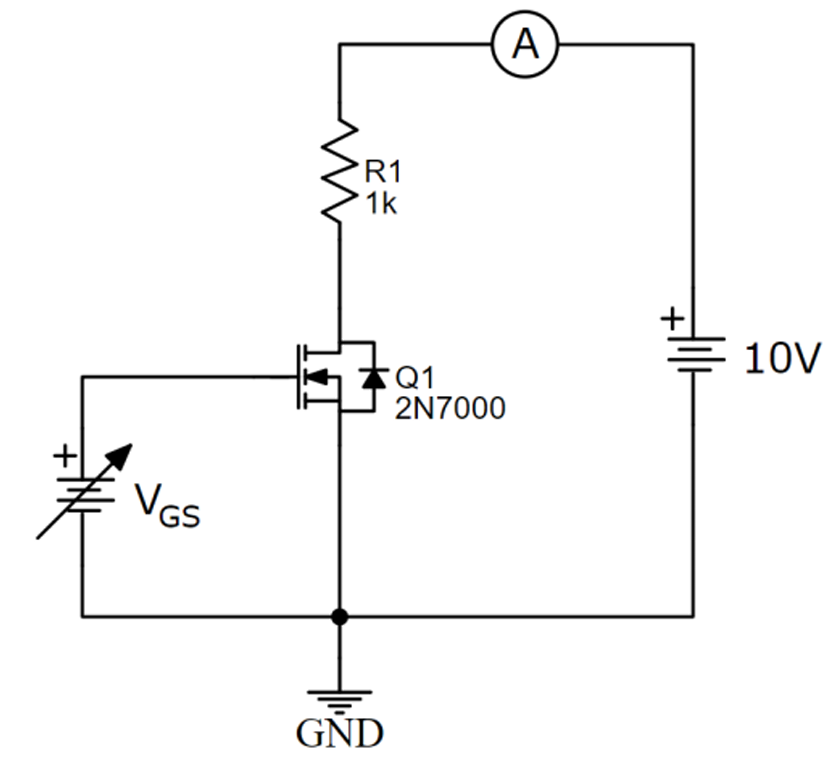
\includegraphics[width=1\linewidth]{fig1.png}

        \textit{Figure 1: Circuit diagram for output characteristics}
    \end{figure}
\end{minipage}\hfill\begin{minipage}{0.55\textwidth}
\begin{enumerate}[leftmargin=*,label=\textbf{\arabic*.}]
\item Test the 2N7000 MOSFET and determine its type.

\item Considering \textit{Figure 1}, take the $V_{GS}$ constant to some value. Vary $V_{DD}$ in steps of $1$ V up to $10$ V and measure the $I_D$. Repeat for $V_{GS} = 1.4, 1.6, \ldots, 2.2\text{ V}$. Obtain the $I_D-V_{DS}$ characteristics.
\end{enumerate}
\end{minipage}

\vspace{1em}

\begin{minipage}{0.4\textwidth}
    \begin{figure}[H]
        \centering
        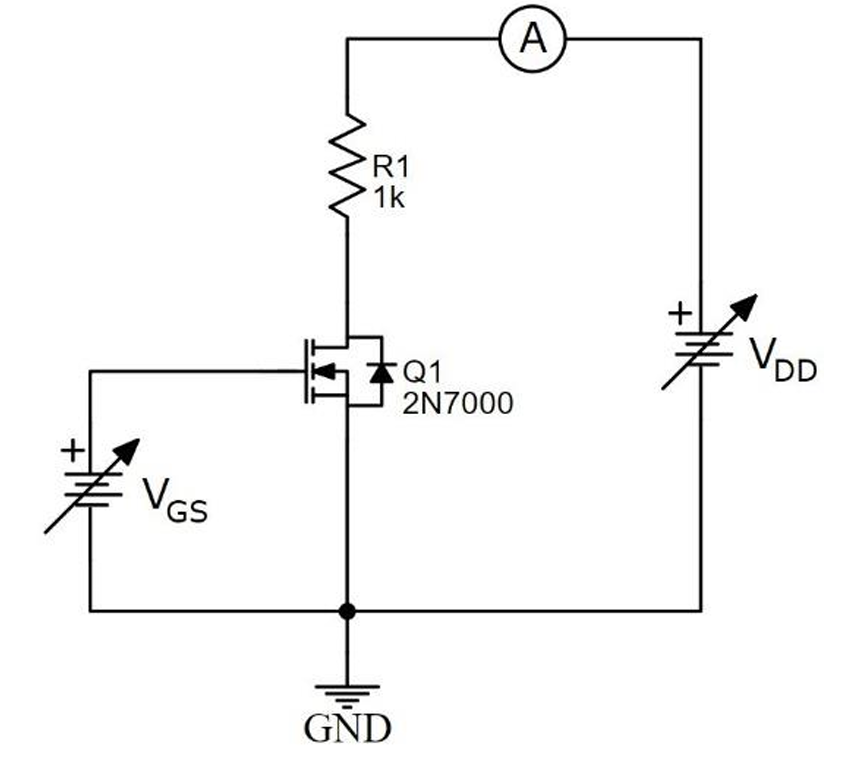
\includegraphics[width=1\linewidth]{fig2.png}

        \textit{Figure 2: Circuit diagram for transfer characteristics} 
    \end{figure}
\end{minipage}\hfill\begin{minipage}{0.55\textwidth}
\begin{enumerate}[leftmargin=*,label=\textbf{\arabic*.}]
\setcounter{enumi}{2}

\item Considering \textit{Figure 2}, obtain the $I_D-V_{GS}$ characteristics. Vary $V_{GS}$ in the step of $0.2$ V up to $2.4$ V and measure the $I_D$. Set the $V_{DD} = 10$ V. Observe the critical point ($V_{TH}$).
\end{enumerate}
\end{minipage}

\section{Answers}

\begin{enumerate}[leftmargin=*,label=\textbf{\arabic*.}]

\item The type of a MOSFET can be identified by using a digital multimeter in diode test mode to check the internal body diode between the drain and source terminals. In an n-channel MOSFET, the body diode conducts when the red probe is connected to the source and the black probe to the drain, while in a p-channel MOSFET conduction occurs when the red probe is connected to the drain and the black probe to the source.

To test whether the MOSFET is defective, the resistance between the terminals is checked. The gate should be insulated from both the drain and source, showing very high resistance. A low resistance between gate and source or between drain and source usually indicates a faulty MOSFET. The switching action can also be tested by charging the gate and observing whether the drain-source resistance changes from high (OFF state) to low (ON state). If the MOSFET fails to switch properly or remains permanently shorted or open, it is defective.

\item The graph is given below.

\begin{center}
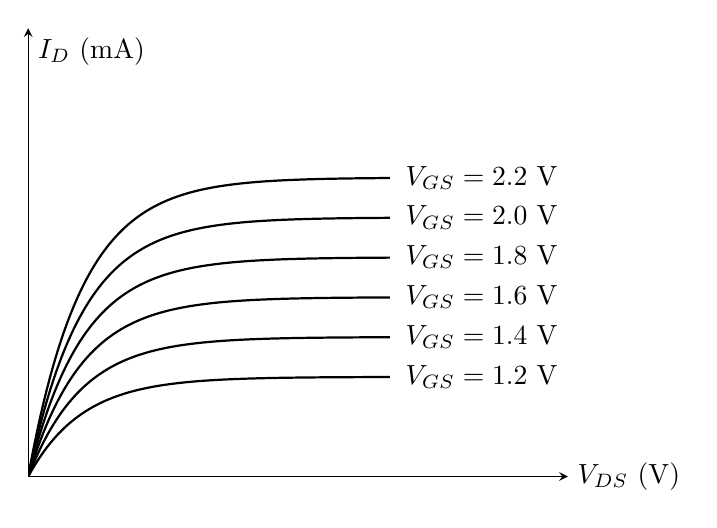
\begin{tikzpicture}
\begin{axis}[
    axis lines=center,
    xlabel={$V_{DS}$ (V)},
    xlabel style={at={(axis description cs:1,0)}, anchor=west},
    ylabel={$I_{D}$ (mA)},
    xmin=0, xmax=10,
    ymin=0, ymax=9,
    xtick=\empty,
    ytick=\empty,
]

\addplot[domain=0:6.7, samples=200, thick] {6*(1 - exp(-x))};
\addplot[domain=0:6.7, samples=200, thick] {5.2*(1 - exp(-x))};
\addplot[domain=0:6.7, samples=200, thick] {4.4*(1 - exp(-x))};
\addplot[domain=0:6.7, samples=200, thick] {3.6-3.6*exp(-x)};
\addplot[domain=0:6.7, samples=200, thick] {2.8-2.8*exp(-x)};
\addplot[domain=0:6.7, samples=200, thick] {2-2*exp(-x)};

\node at (axis cs: 8.4, 2) {$V_{GS}=1.2$~V};
\node at (axis cs: 8.4, 2.8) {$V_{GS}=1.4$~V};
\node at (axis cs: 8.4, 3.6) {$V_{GS}=1.6$~V};
\node at (axis cs: 8.4, 4.4) {$V_{GS}=1.8$~V};
\node at (axis cs: 8.4, 5.2) {$V_{GS}=2.0$~V};
\node at (axis cs: 8.4, 6) {$V_{GS}=2.2$~V};

\end{axis}
\end{tikzpicture}

\small \textit{Graph 2: Transfer characteristics for the given voltages}
\end{center}

\item The expected graph is given below.

\begin{center}
\begin{tikzpicture}
\begin{axis}[
    axis lines=center,
    xlabel={$V_{GS}$ (V)},
    xlabel style={at={(axis description cs:1,0)}, anchor=west},
    ylabel={$I_{D}$ (mA)},
    xmin=0, xmax=16,
    ymin=-1, ymax=9,
    xtick=\empty,
    ytick=\empty,
]

\addplot[domain=7.4:12, samples=200, thick] {exp((x-7.4)/3)-1};
\addplot[domain=12:16, samples=200, thick] {-exp((-x+12))+4.633};

\node at (axis cs: 7.4, -0.5) {$V_{TH}\approx1.6$~V};

\end{axis}
\end{tikzpicture}

\small \textit{Graph 3: Output characteristics for the given voltages}
\end{center}

\end{enumerate}

\textbf{Simulation}

\vspace{1em}

\noindent Since the model isn't included in LTspice internally, the directive \verb|.model 2N7000 VDMOS(Rg=3 Vto=1.6 Rd=0 Rs=.75 Rb=.14 Kp=.17 mtriode=1.25| \verb|Cgdmax=80p Cgdmin=12p Cgs=50p Cjo=50p Is=.04p mfg=Fairchild Vds=60 Ron=2| \verb| Qg=1.5n)| is used.

\newpage

\begin{enumerate}[leftmargin=*,label=\textbf{\arabic*.}]

\item An AC source is applied between the source and drain terminals.

\begin{minipage}{0.45\textwidth}
    \begin{figure}[H]
        \centering
        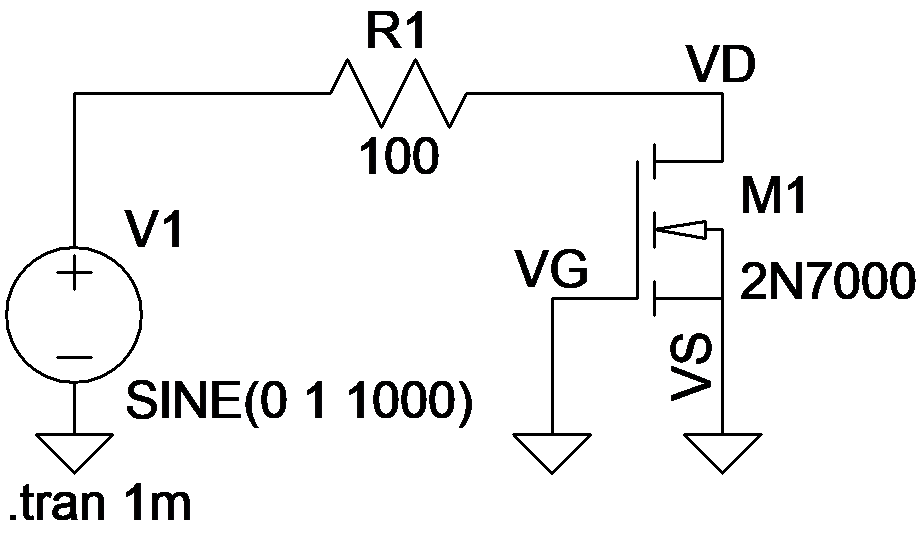
\includegraphics[width=1\linewidth]{fig3.png}

        \textit{Figure 3: MOSFET Defect Test Circuit} 
    \end{figure}
\end{minipage}\hfill\begin{minipage}{0.45\textwidth}

\begin{figure}[H]
    \centering
    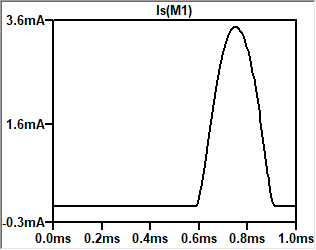
\includegraphics[width=1\linewidth]{fig4.png}

    \textit{Figure 4: Source Current in the Test} 
\end{figure}

\end{minipage}

\vspace{1em}

As expected, the MOSFET is working properly.

\item Since the source is grounded, we can measure the drain voltage. directly.

\begin{figure}[H]
    \centering
    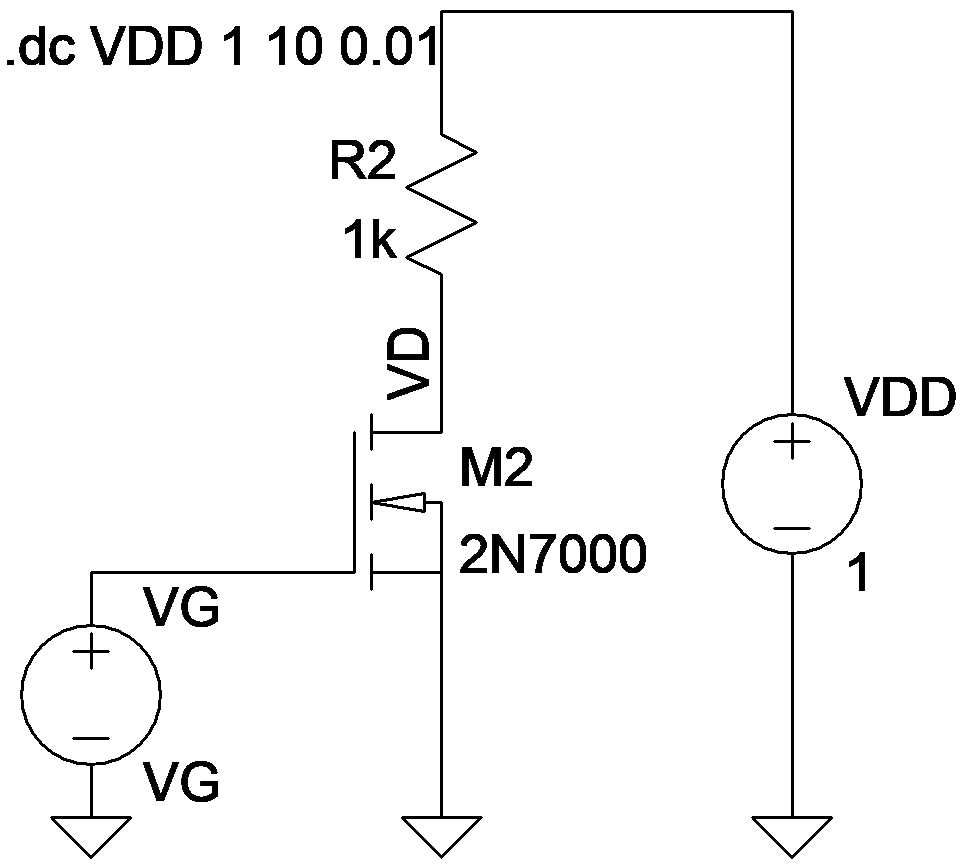
\includegraphics[width=0.4\linewidth]{fig5.png}

    \textit{Figure 5: Adjusted Circuit} 
\end{figure}

\begin{minipage}{0.45\textwidth}
    \begin{figure}[H]
        \centering
        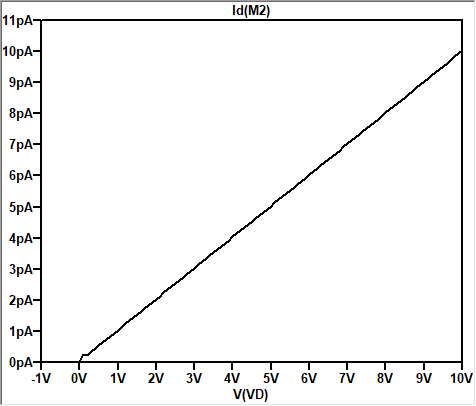
\includegraphics[width=1\linewidth]{1.4.png}

    \textit{Figure 6: Drain Current for $V_{GS}=1.4$}~V
    \end{figure}
\end{minipage}\hfill\begin{minipage}{0.45\textwidth}

\begin{figure}[H]
    \centering
    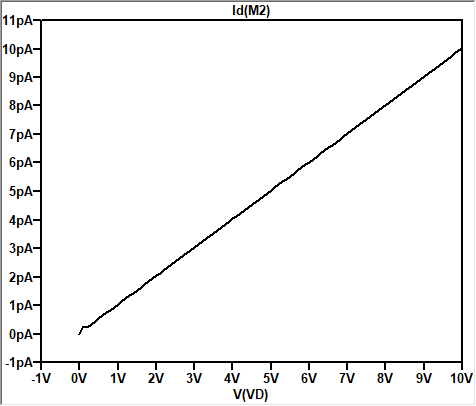
\includegraphics[width=1\linewidth]{1.6.png}

    \textit{Figure 7: Drain Current for $V_{GS}=1.6$}~V
\end{figure}

\end{minipage}

\begin{minipage}{0.45\textwidth}
    \begin{figure}[H]
        \centering
        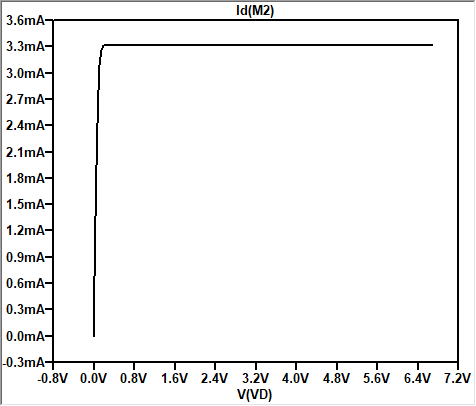
\includegraphics[width=1\linewidth]{1.8.png}

    \textit{Figure 8: Drain Current for $V_{GS}=1.8$}~V
    \end{figure}
\end{minipage}\hfill\begin{minipage}{0.45\textwidth}

\begin{figure}[H]
    \centering
    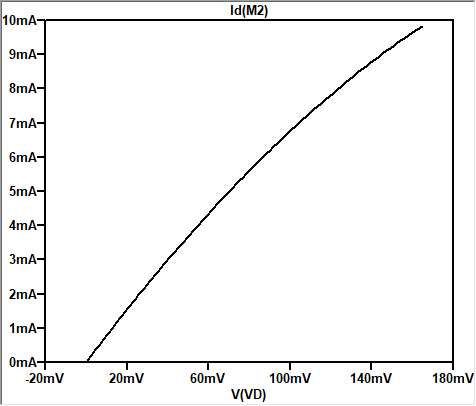
\includegraphics[width=1\linewidth]{2.0.png}

    \textit{Figure 9: Drain Current for $V_{GS}=2.0$}~V
\end{figure}

\end{minipage}

\begin{figure}[H]
    \centering
    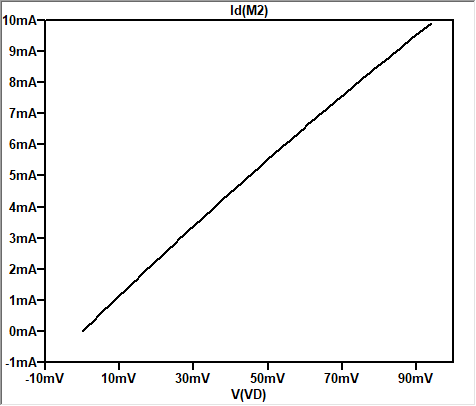
\includegraphics[width=0.45\linewidth]{2.2.png}

    \textit{Figure 10: Drain Current for $V_{GS}=2.2$}~V
\end{figure}

\begin{table}[H]
\centering

\textit{Table 1: $V_{DS}$} ({V}) \textit{and $I_D$} (mA) \textit{values}

\vspace{1em}

\renewcommand{\arraystretch}{1.5} % Adds vertical padding for readability
{\small
\begin{tabular}{|*{10}{c|}}
\hline
\multicolumn{2}{|c|}{$V_{GS}=1.4$~V} & \multicolumn{2}{c|}{$V_{GS}=1.6$~V} & \multicolumn{2}{c|}{$V_{GS}=1.8$~V} & \multicolumn{2}{c|}{$V_{GS}=2$~V} & \multicolumn{2}{c|}{$V_{GS}=2.2$~V} \\ \hline
$V_{DS}$ & $I_D$ & $V_{DS}$ & $I_D$ & $V_{DS}$ & $I_D$ & $V_{DS}$ & $I_D$ & $V_{DS}$ & $I_D$ \\ \hline
0 & 0 & 0&0 &0 & 0& 0& 0& 0& 0\\ \hline
1 & $1.0\cdot10^{-9}$ & 1&$1.0\cdot10^{-9}$ &1 & 0.97& 1&  0.99 & 1& 0.99\\ \hline
 2& $2.0\cdot10^{-9}$ & 2&$2.0\cdot10^{-9}$ & 2& 1.94& 2& 1.97 & 2&1.98 \\ \hline
 3& $3.0\cdot10^{-9}$ & 3& $3.0\cdot10^{-9}$& 3& 2.89& 3& 2.96& 3&2.97 \\ \hline
 4& $4.0\cdot10^{-9}$& 4& $4.0\cdot10^{-9}$& 4& 3.32& 4& 3.95 & 4&3.96 \\ \hline
 5& $5.0\cdot10^{-9}$& 5& $5.0\cdot10^{-9}$& 5& 3.32& 5& 4.93 & 5&4.96\\ \hline
 6& $6.0\cdot10^{-9}$& 6& $6.0\cdot10^{-9}$& 6& 3.32& 6&5.91 & 6&5.95 \\ \hline
 7& $7.0\cdot10^{-9}$& 7& $7.0\cdot10^{-9}$& 7& 3.32& 7&6.90 & 7& 6.94\\ \hline
 8& $8.0\cdot10^{-9}$& 8&$8.0\cdot10^{-9}$ & 8& 3.32& 8& 7.88& 8& 7.93\\ \hline
 9& $9.0\cdot10^{-9}$& 9& $9.0\cdot10^{-9}$& 9& 3.32& 9& 8.86 & 9&8.92 \\ \hline
 10& $10.0\cdot10^{-9}$ & 10& $10.0\cdot10^{-9}$  & 10& 3.32 & 10 & 9.61& 10& 9.91\\ \hline
\end{tabular}
}
\vspace{1em}

\end{table}


\vspace{1cm}

\item $V_{TH}=1.6$~V. The circuit is given below.

\begin{figure}[H]
    \centering
    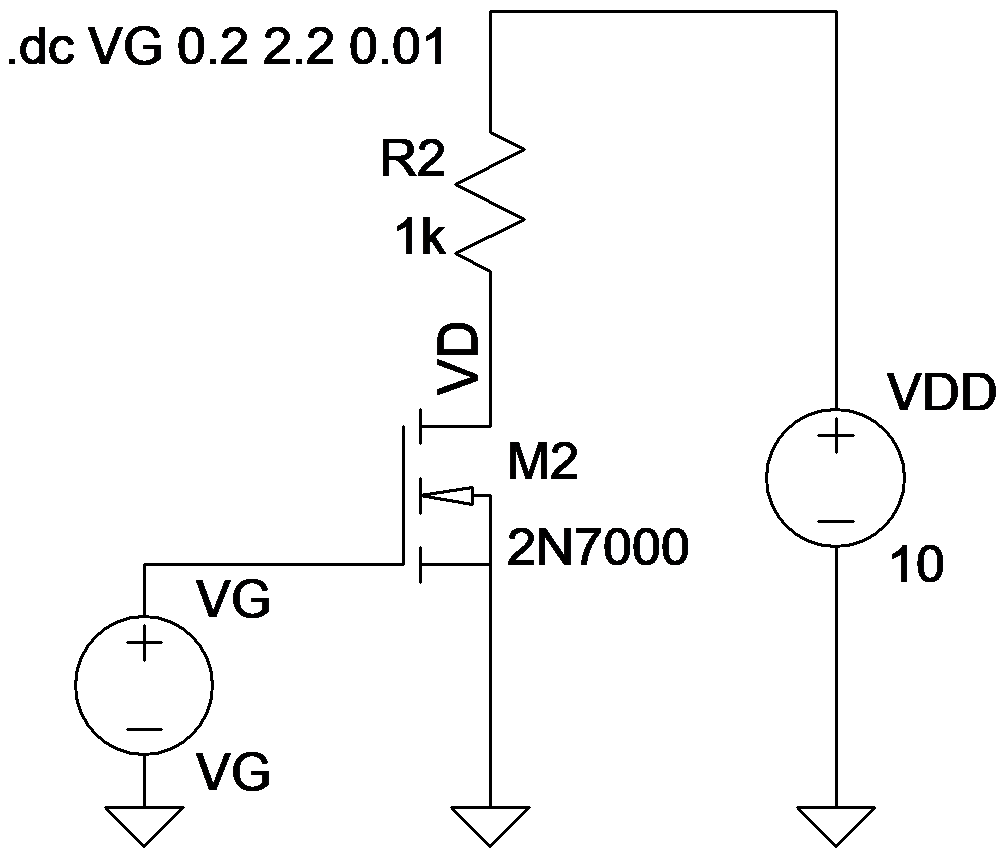
\includegraphics[width=0.5\linewidth]{fig11.png}
    
     \textit{Figure 11: Adjusted Circuit}
\end{figure}

\begin{figure}[H]
    \centering
    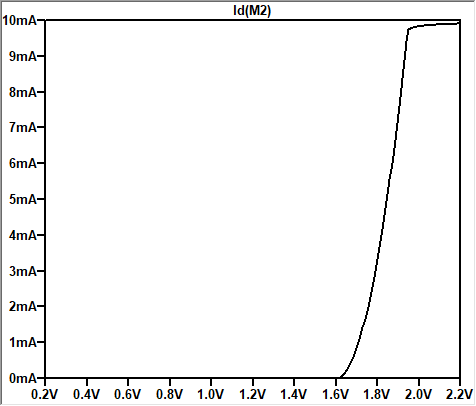
\includegraphics[width=0.5\linewidth]{fig12.png}
    
     \textit{Figure 12: $I_D$--$V_{GS}$ characteristics}
\end{figure}

% --- SECOND TABLE ---
\begin{table}[H]
\centering

\textit{Table 2: \textit{$I_D$ Values for Different Values of $V_{GS}$}}

\vspace{1em}

\renewcommand{\arraystretch}{1.5}
\begin{tabular}{|c|c|*{11}{p{0.60cm}|}}
\hline
 & $V_{GS}$ (V) & 0.2 & 0.4 & 0.6 & 0.8 & 1.0 & 1.2 & 1.4 & 1.6 & 1.8 & 2.0 & 2.2 \\ \cline{2-13}
$V_{DD}=10$~V & $I_D$ (mA) &$10^{-8}$ &$10^{-8}$ & $10^{-8}$ & $10^{-8}$ & $10^{-8}$ &$10^{-8}$ & $10^{-8}$ & $10^{-8}$& 3.32 & 9.84& 9.91 \\ \hline
\end{tabular}
\end{table}

\end{enumerate}
\end{document}